%% LyX 2.3.6.1 created this file.  For more info, see http://www.lyx.org/.
%% Do not edit unless you really know what you are doing.
%\documentclass[11pt,a4paper,english]{desearticle}
\documentclass[11pt,a4paper,english]{desearticle_1col}
\usepackage{mathptmx}
\usepackage{helvet}
\usepackage{courier}
\renewcommand{\familydefault}{\rmdefault}
\usepackage[latin9]{inputenc}
\usepackage{fancyhdr}
\pagestyle{fancy}
\usepackage{mathtools}
\usepackage{graphicx}
\usepackage{esint}

\makeatletter

%%%%%%%%%%%%%%%%%%%%%%%%%%%%%% LyX specific LaTeX commands.
\special{papersize=\the\paperwidth,\the\paperheight}


%%%%%%%%%%%%%%%%%%%%%%%%%%%%%% Textclass specific LaTeX commands.
\newenvironment{lyxlist}[1]
	{\begin{list}{}
		{\settowidth{\labelwidth}{#1}
		 \setlength{\leftmargin}{\labelwidth}
		 \addtolength{\leftmargin}{\labelsep}
		 \renewcommand{\makelabel}[1]{##1\hfil}}}
	{\end{list}}

%%%%%%%%%%%%%%%%%%%%%%%%%%%%%% User specified LaTeX commands.
\Author{Ankit Verma}
\Afil{DESE, IISc}
\Journal{Mechatronic Systems Design}
\Month{Aug-Dec}
\Year{2021}

\makeatother

\usepackage{babel}
\begin{document}
\title{{\huge{}Exercise 1}}
\title{Exercise 1 : Modelling}
\author{Ankit Verma}
\maketitle

\section*{Answer for system A:}

Let us consider the mass is M, coefficient of spring stiffness is
k and coefficient of damper is b.
\begin{figure}
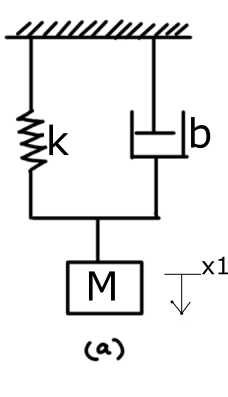
\includegraphics[bb=0bp 0bp 171bp 298bp,scale=0.4]{img11}\caption{System A}
\end{figure}


\subsection*{Task1:}

Energy Variables
\begin{itemize}
\item $\frac{1}{2}M$($\frac{dx_{1}}{dt})^{2}$
\item $\frac{1}{2}kx_{1}^{2}$
\end{itemize}

\subsection*{Task 2:}

List of state variables
\begin{itemize}
\item $x_{1}$
\item $x_{2}$
\end{itemize}

\subsection*{Task 3:}

\subsubsection*{State equations}
\begin{lyxlist}{00.00.0000}
\item [{$\mathllap{\mathllap{}}\frac{dx_{1}}{dt}=x_{2}$}]~
\item [{$\Rightarrow\dot{x}_{1}=x_{2}$}]~
\item [{$\mathllap{\mathllap{}}M\frac{d^{2}x_{1}}{dt^{2}}+b\frac{dx_{1}}{dt}+kx_{1}=0$}]~
\item [{$\Rightarrow\frac{d^{2}x_{1}}{dt^{2}}+\frac{b}{M}\frac{dx_{1}}{dt}+\frac{k}{M}x_{1}=0$}]~
\item [{$\Rightarrow\frac{dx_{2}}{dt}+\frac{b}{M}\frac{dx_{1}}{dt}+\frac{k}{M}x_{1}=0$}]~
\item [{$\Rightarrow\frac{dx_{2}}{dt}=-\frac{b}{M}\frac{dx_{1}}{dt}-\frac{k}{M}x_{1}$}]~
\item [{$\Rightarrow\dot{x}_{2}=-\frac{b}{M}\dot{x}_{1}-\frac{k}{M}x_{1}$}]~
\end{lyxlist}

\section*{Answer for system B:}

\begin{figure}
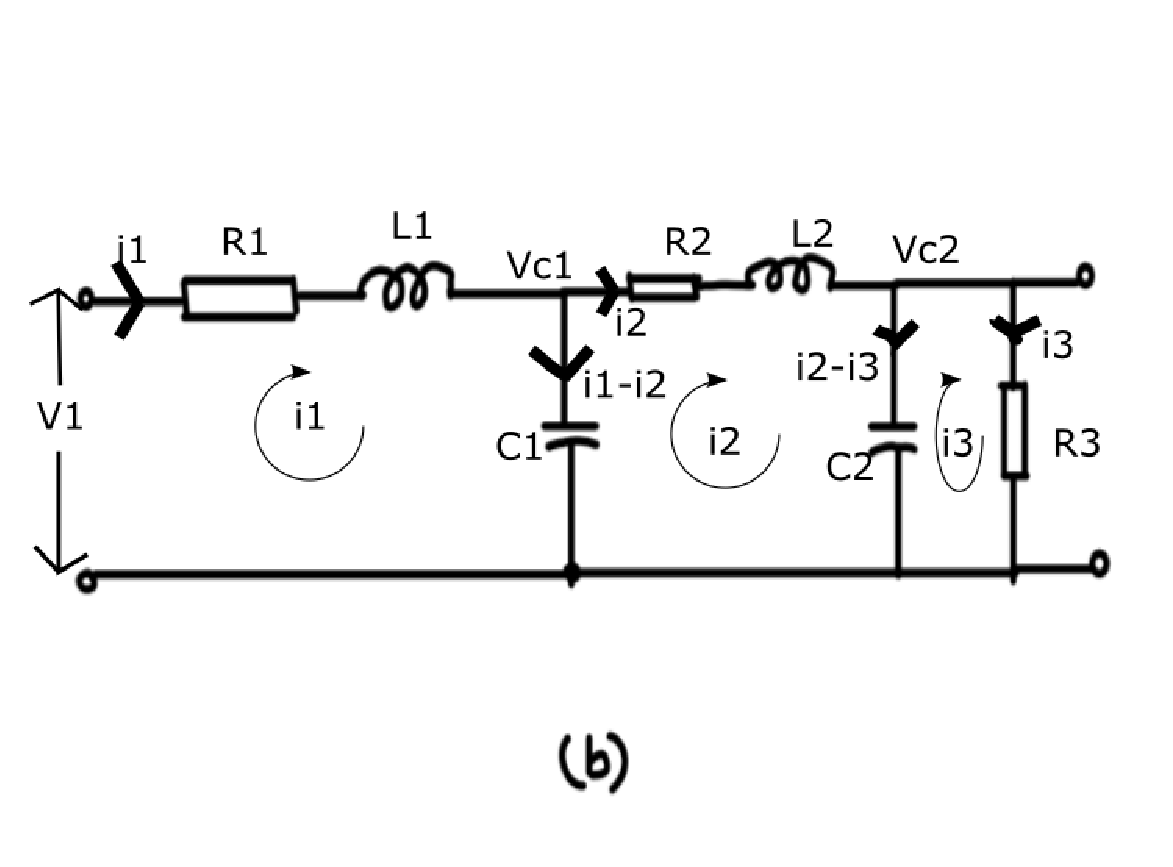
\includegraphics[scale=0.5]{img22}\caption{System B}
\end{figure}


\subsection*{Task 1:}

Energy Variables
\begin{itemize}
\item $\frac{1}{2}L_{1}i_{1}^{2}$
\item $\frac{1}{2}L_{2}i_{2}^{2}$
\item $\frac{1}{2}C_{1}V_{C1}^{2}$
\item $\frac{1}{2}C_{2}V_{C2}^{2}$
\end{itemize}

\subsection*{Task 2:}

List of state variables
\begin{enumerate}
\item $i_{1}$
\item $i_{2}$
\item $V_{C1}$
\item $V_{C2}$
\end{enumerate}

\subsection*{Task 3:}

\subsubsection*{State equation}

Applying KVL in Loop i1:
\begin{lyxlist}{00.00.0000}
\item [{$V_{1}-i_{1}R_{1}-L_{1}\frac{di_{1}}{dt}-V_{C_{1}}=0$}]~
\item [{$\Rightarrow\frac{di_{1}}{dt}=\frac{V_{1}}{L_{1}}-\frac{V_{C_{1}}}{L_{1}}-\frac{i_{1}R_{1}}{L_{1}}$}]~
\item [{$\Rightarrow\dot{i}_{1}=\frac{V_{1}}{L_{1}}-\frac{V_{C_{1}}}{L_{1}}-\frac{i_{1}R_{1}}{L_{1}}$}]~
\end{lyxlist}
At node Vc1:
\begin{lyxlist}{00.00.0000}
\item [{$V_{C_{1}}=\frac{1}{C_{1}}\int(i_{1}-i_{2})dt$}]~
\end{lyxlist}
Differentiating both side with respect to $t$
\begin{lyxlist}{00.00.0000}
\item [{$\Rightarrow\frac{dV_{C_{1}}}{dt}=\frac{i_{1}}{C_{1}}-\frac{i_{2}}{C_{1}}$}]~
\item [{$\Rightarrow\dot{V}_{C_{1}}=\frac{i_{1}}{C_{1}}-\frac{i_{2}}{C_{1}}$}]~
\end{lyxlist}
Applying KVL in Loop i2:
\begin{lyxlist}{00.00.0000}
\item [{$V_{C_{1}}-i_{2}R_{2}-L_{2}\frac{di_{2}}{dt}-V_{C_{2}}=0$}]~
\item [{$\Rightarrow\frac{di_{2}}{dt}=\frac{V_{C_{1}}}{L_{2}}-\frac{V_{C_{2}}}{L_{2}}-\frac{i_{2}R_{2}}{L_{2}}$}]~
\item [{$\Rightarrow\dot{i}_{2}=\frac{V_{C_{1}}}{L_{2}}-\frac{V_{C_{2}}}{L_{2}}-\frac{i_{2}R_{2}}{L_{2}}$}]~
\end{lyxlist}
At node Vc2:
\begin{lyxlist}{00.00.0000}
\item [{$V_{C_{2}}=\frac{1}{C_{2}}\int(i_{2}-i_{3})dt$}]~
\end{lyxlist}
Differentiating both side with respect to $t$
\begin{lyxlist}{00.00.0000}
\item [{$\Rightarrow\frac{dV_{C_{2}}}{dt}=\frac{i_{2}}{C_{2}}-\frac{i_{3}}{C_{2}}$}]~
\item [{$\Rightarrow\frac{dV_{C_{2}}}{dt}=\frac{i_{2}}{C_{2}}-\frac{V_{C_{2}}}{R_{3}C_{2}}$}] as
$i_{3}=\frac{V_{C_{2}}}{R_{3}}$
\item [{$\Rightarrow\dot{V}_{C_{2}}=\frac{i_{2}}{C_{2}}-\frac{V_{C_{2}}}{R_{3}C_{2}}$}]~
\end{lyxlist}

\section*{Answer for system C:}

\begin{figure}
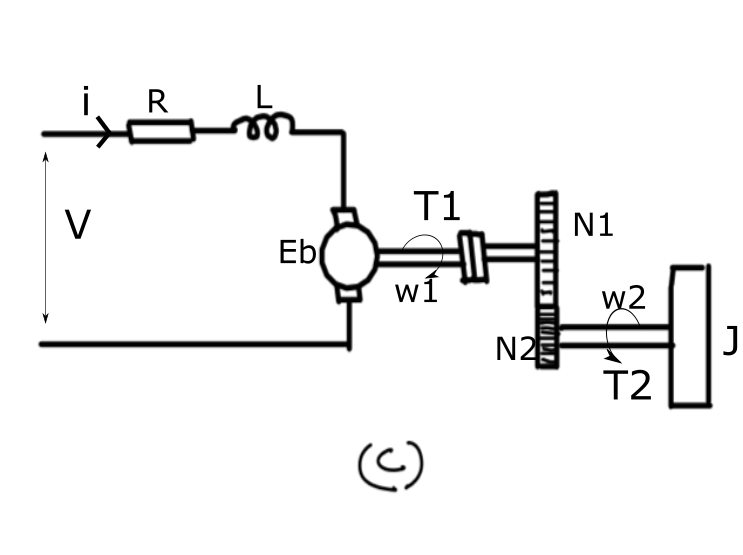
\includegraphics[scale=0.5]{img33}\caption{System C}
\end{figure}


\subsection*{Task 1:}

Energy Variables
\begin{itemize}
\item $\frac{1}{2}Li^{2}$
\item $\frac{1}{2}Jw_{1}^{2}$
\end{itemize}

\subsection*{Task 2:}

List of state variables
\begin{itemize}
\item $i$
\item $\omega_{2}$
\end{itemize}

\subsection*{Task 3:}

Let us assume $E_{b}$is back EMF of the motor and J is the moment
of inertia of the flywheel.
\begin{lyxlist}{00.00.0000}
\item [{$E_{b}=k\omega_{1}$}]~
\end{lyxlist}

\subsubsection*{State equation}

Now considering the gear ratio is $N_{1}:N_{2}$ so the speed would
be $\omega_{1}$:$\omega_{2}$. Now, the torque developed by the motor
is given by
\begin{lyxlist}{00.00.0000}
\item [{$T_{1}=k_{m}i$}] {[}considering flux constant{]}
\end{lyxlist}
The torque transformed to flywheel side will be given by
\begin{lyxlist}{00.00.0000}
\item [{$T_{2}=\frac{T_{1}N_{1}}{N_{2}}$}]~
\item [{Or}]~
\item [{$T_{1}\omega_{1}=T_{2}\omega_{2}$}]~
\item [{$\Rightarrow\omega_{1}=\frac{T_{2}\omega_{2}}{T_{1}}$}]~
\end{lyxlist}
which is also given by
\begin{lyxlist}{00.00.0000}
\item [{T$_{2}=J\frac{d\omega_{2}}{dt}$}]~
\end{lyxlist}
So,
\begin{lyxlist}{00.00.0000}
\item [{$\frac{d\omega_{2}}{dt}=\frac{T_{1}N_{1}}{JN_{2}}$}]~
\item [{$\Rightarrow\frac{d\omega_{2}}{dt}=\frac{k_{m}N_{1}i}{JN_{2}}$}]~
\item [{$\Rightarrow\dot{\omega}_{2}=\frac{k_{m}N_{1}i}{JN_{2}}$}]~
\end{lyxlist}
Apllying KVL in the electrical motor circuit loop
\begin{lyxlist}{00.00.0000}
\item [{$V=iR+L\frac{di}{dt}+E_{b}$}]~
\item [{$\Rightarrow\frac{di}{dt}=\frac{V}{L}-\frac{iR}{L}-\frac{k\omega_{1}}{L}$}]~
\item [{$\Rightarrow\dot{i}=\frac{V}{L}-\frac{iR}{L}-\frac{kT_{2}\omega_{2}}{T_{1}L}$}]~
\end{lyxlist}

\end{document}
